\documentclass[11pt, a4paper]{article}

% Encoding
\usepackage[utf8]{inputenc}

% Hyphenation
\usepackage[english]{babel}

% Extended math environments
\usepackage{amsmath}
\numberwithin{equation}{section}

% Additional math fonts and symbols
\usepackage{amsfonts}
\usepackage{amssymb}

% Units and uncertainties
\usepackage{siunitx}
\sisetup{
    separate-uncertainty
}

% Margins
\usepackage[left=3.5cm, right=3.5cm, top=3cm, bottom=3cm, twoside]{geometry}

% Pictures
\usepackage{graphicx}

% Text color
\usepackage{color}

% Hyperlinks
\usepackage{hyperref}
\hypersetup{
    colorlinks = true,
    allcolors = {black}
}

% Better table layouts
\usepackage{booktabs}
\usepackage{multirow}
\usepackage{multicol}

% Page Header
\usepackage{fancyhdr}

% Float Barriers
\usepackage{placeins}

% Rotated figures
\usepackage{caption}
\usepackage{subcaption}
\usepackage{rotating}

% Wrapped figures
\usepackage{wrapfig}

\usepackage{float}

% Remarks
\newcommand{\remark}[1]{{\color{red}(#1)}}

% Code
\usepackage{listings}
\definecolor{dkgreen}{rgb}{0,0.6,0}
\definecolor{gray}{rgb}{0.5,0.5,0.5}
\definecolor{mauve}{rgb}{0.58,0,0.82}

\lstset{frame=tb,
	aboveskip=3mm,
	belowskip=3mm,
	showstringspaces=false,
	columns=flexible,
	basicstyle={\footnotesize\ttfamily},
	numbers=left,
	numbersep=4pt,
	numberstyle=\tiny\color{black},
	keywordstyle=\color{blue},
	commentstyle=\color{dkgreen},
	stringstyle=\color{mauve},
	breaklines=true,
	breakatwhitespace=true,
	tabsize=4,
	xleftmargin=1em,
	xrightmargin=0.8em
}

% Caption-Setup
\captionsetup{font={small}}
\renewcommand{\thefigure}{\thesection.\arabic{figure}}
\renewcommand{\thesubfigure}{\alph{subfigure}}
\renewcommand{\thetable}{\thesection.\arabic{table}}
\renewcommand{\thesubtable}{\alph{subtable}}

% Depth of TOC (Level: 1 sections, 2 subsections, 3 subsubsections)
\setcounter{tocdepth}{3}

% FANCYHDR SETUP
\pagestyle{fancy}
\fancyhead[EL,OR]{\thepage}
\fancyhead[ER]{\leftmark}
\fancyhead[OL]{\rightmark}

\renewcommand{\sectionmark}[1]{
\markboth{\thesection{} #1}{\thesection{} #1}
}
\renewcommand{\subsectionmark}[1]{
\markright{\thesubsection{} #1}
}

% Document Info
\title{Particles in a potential}

\author{Christopher Deutsch\footnote{christopher.deutsch@uni-bonn.de} \and Philip Hauer\footnote{philiphauer@googlemail.com}}

\date{\today}

\begin{document}

\begin{titlepage}

\maketitle

% ABSTRACT
\begin{abstract}
\noindent 
A set of two oppositely charged particles that interact via a two-particle potential in a finite volume in two dimensions is considered.
With a Random-Walk Metropolis algorithm one can simulate the time evolution of this system.
The focus of this report lies on the analysis of the temperature dependence in particular the average pair-distance.
Additionally the behavior for different potentials and in three dimensions is also studied.
\end{abstract}

\end{titlepage}

% TABLE OF CONTENTS
\tableofcontents
% New page after TOC
\newpage

% CONTENT

\section{Introduction}
This report summarizes the results of the analysis of a two-dimensional system where only two kind of particles, a positive and a negative one are considered.
They interact via a potential which is given by
\begin{equation}
V_{ij} = \frac{q_i q_j}{\left| \vec{r}_i - \vec{r}_j \right|} + \frac{1}{\left| \vec{r}_i - \vec{r}_j \right|^8} \, \text{.} \label{Eq:Potential}
\end{equation}
For the analysis a Random-Walk Metropolis algorithm is used. It will be explained in section \ref{sec:Metropolis}.
The used algorithm depends on the temperature and this dependence is studied in section \ref{sec:Temperature}.
As an indicator for the phase of the system the average pair-distance is monitored.
A visualization of the different phases was also done and can be found in the section \ref{sec:Visualisation}.
In addition to that some further researches with other potentials (e.g. Lennard-Jones potential) were done and the behavior of this system in three dimensions was also analyzed.
These further thoughts and results are explained in section \ref{sec:Further_Analysis}.


\section{Background}

\subsection{Canonical ensemble} \label{sec:Canonical_Ensemble}
\begin{wrapfigure}[14]{o}[20pt]{0.45\textwidth}
	\centering
	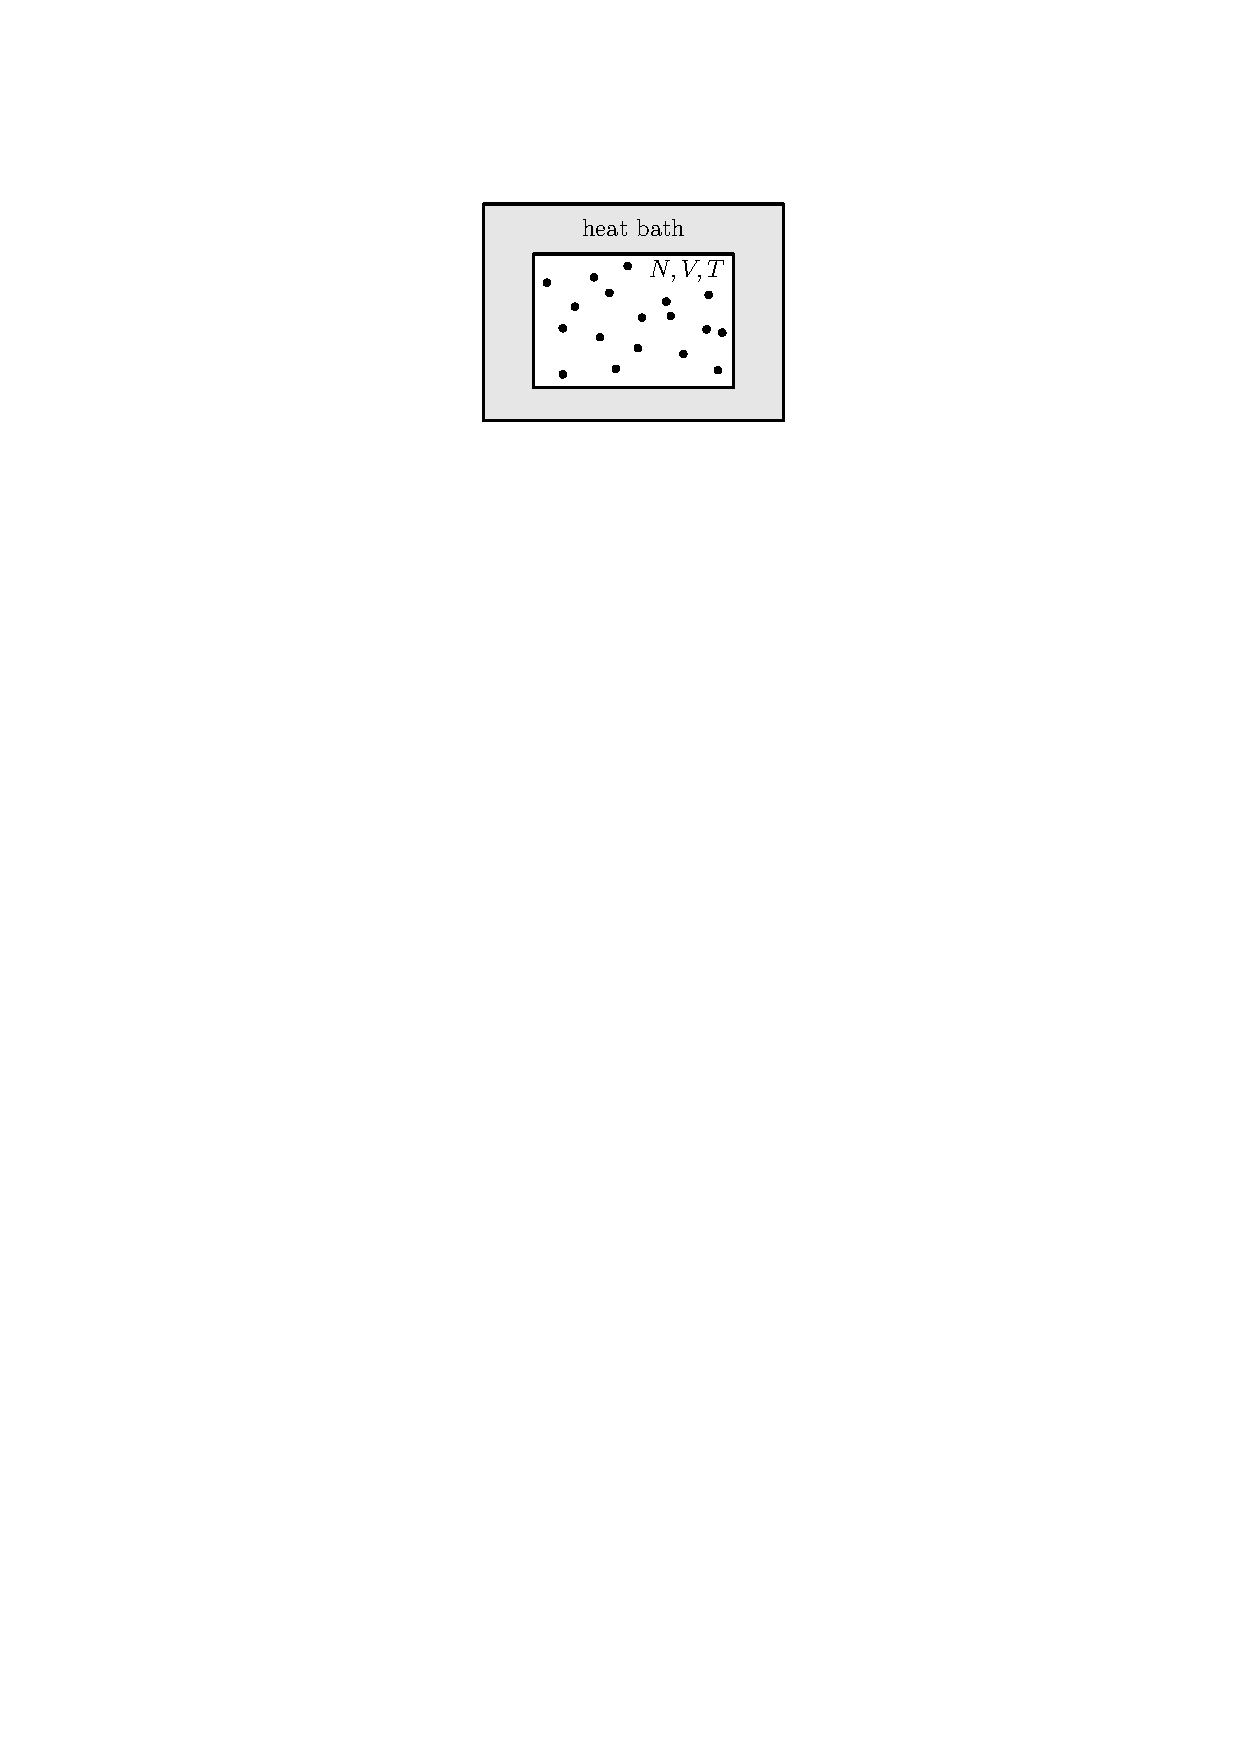
\includegraphics[width=0.4\textwidth]{./figures/canonical_ensemble.pdf}
	\caption{Schematic representation of the canonical ensemble.}
	\label{fig:canonical_ensemble}
\end{wrapfigure}
The statistical ensemble describing a fixed number of particles~$N$ in a given volume~$V$, which is in thermal equilibrium with a heat bath of temperature~$T$, is the canonical ensemble (cf.\ figure \ref{fig:canonical_ensemble}).
Aim of this project is to sample states from a given ensemble with fixed $N, V, T$ and use these to calculate expectation values of certain observables.
For this the probability density for realizing a specific microstate of the ensemble needs to be known.
In statistical mechanics the probability density for a canonical ensemble to be in a microstate with energy eigenvalue~$E$ is given by \cite{schwabl}
\begin{align*}
	P = \frac{1}{Z} \exp\left[ -\beta E \right] \qquad \beta := \frac{1}{k_\mathrm{B} T}
\end{align*}
with the normalization factor $1/Z$, where $Z$ is the canonical partition function.
For a system of particles with an inter-particle potential~$V_{ij}$ and neglecting kinetic energies the canonical partition function
\begin{align*}
	Z = \int \prod_{i=1}^N \mathrm{d}\mathbf{r}_i \exp\left[ -\beta \sum_{i < j} V_{ij} \right]
\end{align*}
is a constant of the ensemble and the total energy of the system is
\begin{align*}
	E = \sum_{i < j} V_{ij} \, \text{.}
\end{align*}
Since the calculation of $Z$ is computationally expensive a sampling method without the need of a normalized probability density is desirable.
One such method is sampling using the Metropolis algorithm, which is introduced in the following section.


\subsection{Metropolis algorithm} \label{sec:Metropolis}
The Metropolis algorithm is a Markov-chain Monte-Carlo method for generating an autocorrelated sequence of random samples of a given probability distribution.
These samples can be used to approximate distributions for which direct sampling methods cannot be employed.
Hereafter a summary of the algorithm is given.\\

\noindent\textbf{Random-Walk Metropolis algorithm:}\\
For a given initial state~$x_0$ and target density~$P(x)$, a sequence of random samples~$\left( x_n \right)$ can be obtained using the following steps:
\begin{enumerate}
	\item \textbf{Trial change:}
		Propose a new state $y$ according to a symmetric proposal distribution $q(Y|x_n)$ depending on the current state $x_n$.
		
	\item \textbf{Accept-reject step:}
		Calculate the acceptance probability
		\begin{align*}
			\alpha(x, y) = \min\left\{ \frac{P(y)}{P(x_n)}, 1\right\} \,\text{.}
		\end{align*}
		Generate $u \sim \mathcal{U}(0, 1)$ and set the random sample~$x_{n+1}$ according to:
		\begin{align*}
			x_{n+1} = \begin{cases}
					y_n \,, & u \leq \alpha(x_n, y_n) \\
					x_n \,, & u > \alpha(x_n, y_n)
				\end{cases}
		\end{align*}
		
	\item \textbf{Repeat}
\end{enumerate}
Moreover the target density~$P(x)$ does not need to be normalized, since it only occurs as a fraction of densities in the accept-reject step.
Therefore this algorithm is suitable to sample from a canonical ensemble without the explicit calculation of the canonical partition function.

Finally one has to consider the influence of the proposal scheme on the behavior of the algorithm.
A characteristic indicator of this is the mean acceptance rate in the accept-reject step.
Generally, a small acceptance rate leads to slow mixing of the Markov-Chain, which means, that the state moves slowly through state-space.
Conversely a high acceptance gives rise to rapid mixing of the chain and a thorough exploration of the state-space.
In addition to this, the algorithm is less likely to get stuck at a local mode of the target distribution.
In practice one has to balance both effects to achieve optimal performance of the algorithm.
It is suggested \cite{gilks_richardson}, that a mean acceptance rate in the interval~$[0.15, 0.5]$ leads to good performance.

\section{Implementation} \label{sec:implementation}
For the simulations of the canonical ensemble the programming language \texttt{C++} was used.
In the following a summary of the core implementation details is given.

\subsection{Metropolis algorithm} \label{sec:Metropolis_alg}
Since the subject of this project requires the simulation of particles in two or three dimensions and different inter-particle potentials, a generic approach of implementing the algorithmic core was chosen.
The source code of the implementation is listed in appendix~\ref{sec:canonical_ensemble_source}.

The Metropolis algorithm is encapsulated in a class-template~\texttt{CanonicalEnsemble} taking a parameter \texttt{ParticleState} indicating the type used to describe the state of one particle.
For the case of two-dimensional charged particles this could be a \texttt{struct} containing three floating point members describing the particle charge~$q$ and two coordinates~$x, y$.
Each object of type \texttt{CanonicalEnsemble} has several important (inaccessible) members associated with it:
\begin{itemize}
	\item \texttt{state}:
		A dynamically allocated array of type \texttt{ParticleState} fully describing the state of the ensemble (i.e.\ the charges and coordinates of all particles).
		The current state can be queried using the \texttt{get\_state} member-function.
	
	\item \texttt{beta}:
		The thermodynamic beta~$\beta = (k_\mathrm{B} T)^{-1}$ of the heat bath associated with the canonical ensemble.
	
	\item \texttt{potential\_func}:
		A function object taking two particles and returning their inter-particle potential.
	
	\item \texttt{proposal\_func}:
		A function object taking a particle and a random number generator, which returns a new particle according to a user-defined proposal distribution.
\end{itemize}
These members are assigned at construction-time of a \texttt{CanonicalEnsemble}-object and therefore allow for full customization of the considered problem.
The underlying Metropolis algorithm is implemented in the \texttt{step} member-function:
\lstinputlisting[language=C++, firstline=59, lastline=79]{../code/src/CanonicalEnsemble.h}
In the following a detailed description of the implemented algorithm shall be given.
\begin{enumerate}
	\item
		A random particle of the currently realized state is selected using a uniform distribution of indices.
		The contribution to the total potential energy~$V$ of the chosen particle~$V_j$ is calculated using a helper-function \texttt{potential} according to
		\begin{align*}
			V_j = \sum_{\substack{i = 1 \\ i \neq j}}^N V_{ij}
		\end{align*}
		with the inter-particle potential $V_{ij}$ as specified in \texttt{potential\_func}.
		
	\item
		The state of the selected particle is saved and a trial change of the current state is made using the proposal distribution as implemented in \texttt{proposal\_func} (further details in section \ref{sec:proposal_function}).
		Then the contribution of the proposed particle to the total potential energy~$V$ is calculated.
		
	\item
		At this point the target distribution of the canonical ensemble
		\begin{align*}
			P \propto \exp\left[ - \beta E \right]
		\end{align*}
		with the total energy of the system
		\begin{align*}
			E = \sum_{i < j} V_{ij}
		\end{align*}
		has to be considered.
		To obtain the acceptance probability~$\alpha$ according to equation \eqref{eq:acceptance_probability} the ratio
		\begin{align} \label{Eq:Prob_New_State}
			\alpha = \frac{\exp\left[ -\beta E_\mathrm{prop.} \right]}{\exp \left[ -\beta E_\mathrm{cur.} \right]} = \exp\left[ -\beta \left( E_\mathrm{prop.} - E_\mathrm{cur.} \right) \right]
		\end{align}
		is calculated.
		Since only one particle was changed, the difference $E_\mathrm{prop.} - E_\mathrm{cur.}$ reduces to the difference in contributions to the potential energy of the proposed and the current particle state.
		
		Lastly a $\mathcal{U}(0, 1)$-distributed random variable is compared to the calculated acceptance probability.
		If the variable is smaller than the acceptance probability the trial configuration is rejected, the old state is restored and the member function returns \texttt{false} indicating that the proposed state was rejected.
		Otherwise the new proposed state is kept and \texttt{true} is returned.		
\end{enumerate}

\subsection{Proposal function} \label{sec:proposal_function}
The proposal function contains an implementation of the proposal distribution, which occurs in the Metropolis algorithm.
Its required arguments are a reference to a \texttt{ParticleState} representing the state of one particle, for which a new state according to the proposal distribution should be chosen.
Moreover the function takes a reference to a random number generator, which is used to create random variables for sampling from the proposal distribution.

For illustration purposes consider the one dimensional case of a particle with charge~$q$ and a coordinate~$x$ on a line.
A proposal distribution
\begin{align*}
	q(y|x) = \begin{cases}
		\frac{1}{2\Delta} \,, & y \in \left[x - \Delta, x + \Delta \right]\\
		0 \,, & \text{else}
	\end{cases}
\end{align*}
suggesting a new particle position uniformly on a line segment of length $2\Delta$ centered at the current particle position~$x$.
This could be implemented as a proposal function in the following way:
\begin{lstlisting}[language=C++]
struct Particle1D {
	double q;
	double x;
}

Particle1D proposal_function_1d(const Particle1D &p, std::m19937 &rng) {
	std::uniform_real_distribution<> unif_dist(-delta, delta);
	
	Particle1D ret;
	ret.q = p.q;
	ret.x = p.x + unif_dist(rng);
	
	return ret;
}
\end{lstlisting}
(for this to be valid code the parameter \texttt{delta} must be set\footnote{For the implementation used in this report, proposal functions are realized as function objects with an associated member \texttt{delta}.}).
This scheme is easily extended to charged/uncharged particles in two or three dimensions, using an uniform proposal in a box centered at the particle position.
The simulated data used in this report was generated using such a proposal scheme.


\section{Temperature dependence of the canonical ensemble} \label{sec:Temperature}
To analyze the temperature dependence of the canonical ensemble using different inter-particle potentials, which will be introduced in section \ref{sec:Potentials}, the implementation as described in section~\ref{sec:implementation} is used.
At first some important settings of the simulation, which vary depending on the case considered, shall be introduced.

The initial state of the simulation is a random distribution of~$N$ charged or uncharged particles inside a two or three dimensional box with side length~$L$.
Since a random initial state is unprobable according to the target distribution, a burn-in phase discarding the first 1000 samples of the Markov-Chain will be employed.

For monitoring the phase transitions of the ensemble, the average pair-distance (introduced in section \ref{sec:Temp_Dep}) can be observed over a specific temperature range or more precisely the thermodynamic~$\beta$, which needs to be set beforehand.
As explained in section \ref{sec:Metropolis} the mean acceptance rate is critical for good performance of the algorithm, which strongly depends on the simulated temperature and the parameter~$\Delta$ of the proposal function.
Initial testing of the algorithm showed that reasonable performance can be obtained with an acceptance rate of~\SI{30}{\percent}.
Therefore the parameter~$\Delta$ of the proposal function has to be adapted depending on the considered temperature to achieve the desired acceptance rate.

Despite carefully setting the acceptance rate, the Random-Walk Metropolis algorithm often gets stuck at local modes of the target probability density.
Therefore an approach of simulating a number of shorter chains was chosen.
The chosen parameters of the simulation will be stated in the corresponding sections.

\subsection{Potentials} \label{sec:Potentials}
In the following a short introduction of the inter-particle potentials used in the simulation of the canonical ensemble is given.
For computational simplicity all quantities are considered to be dimensionless and charges are assumed to be $\pm 1$.

\begin{description}
	\item[Coulomb potential with hard core:]
		The Coulomb potential of two charged particles $V_\mathrm{Coulomb} \propto r^{-1}$ and a short ranged force $V_\mathrm{core} \propto r^{-8}$ parameterizing the particle's hard core  is given as
		\begin{align*}
			V_{ij} = \frac{q_i q_j}{| \mathbf{r}_i - \mathbf{r}_j |} + \frac{1}{| \mathbf{r}_i - \mathbf{r}_j |^8}
		\end{align*}
		with particle charges~$q$ and position vectors~$\mathbf{r}$.
		At intermediate ranges this force is attractive for oppositley charged particles and repulsive for particles of the same charge.
		The general behavior of this potential is depicted in figure \ref{fig:coulomb_core} and the hard core of the potential is visible as the steep ascend of the potential energy at a distance of $r \approx 1$.
		Moreover a prominent minimum of the potential for oppositley charged particles can be observed at $r \approx 1.35$.
		This is approximately the lattice spacing of crystals formed at low temperatures, as can be seen in section \ref{sec:2d_coulomb_vis}.
		
	\item[Lennard-Jones potential:]
		The Lennard-Jones potential describes the inter-atomic potential between a pair of neutral atoms interacting via attractive Van der Waals forces $V_\mathrm{VdW} \propto r^{-6}$ and a repulsive contribution due to the Pauli exclusion principle $V_\mathrm{Pauli} \propto r^{-12}$.
		Without loss of generality one can assume the functional form
		\begin{align*}
			V_{ij} = \frac{1}{| \mathbf{r}_i - \mathbf{r}_j |^{12}} - \frac{1}{| \mathbf{r}_i - \mathbf{r}_j |^6} \, \text{.}
		\end{align*}
		This is depicted in figure \ref{fig:lennard_jones} and is similar to the Coulomb potential of oppositley charged particles.
		However the Lennard-Jones potential is extremely short ranged due to its $r^{-6}$-dependence as compared to the $r^{-1}$-dependence of the Coulomb potential.
\end{description}

\begin{figure}[p]
	\begin{subfigure}{1.0\textwidth}
		\centering
		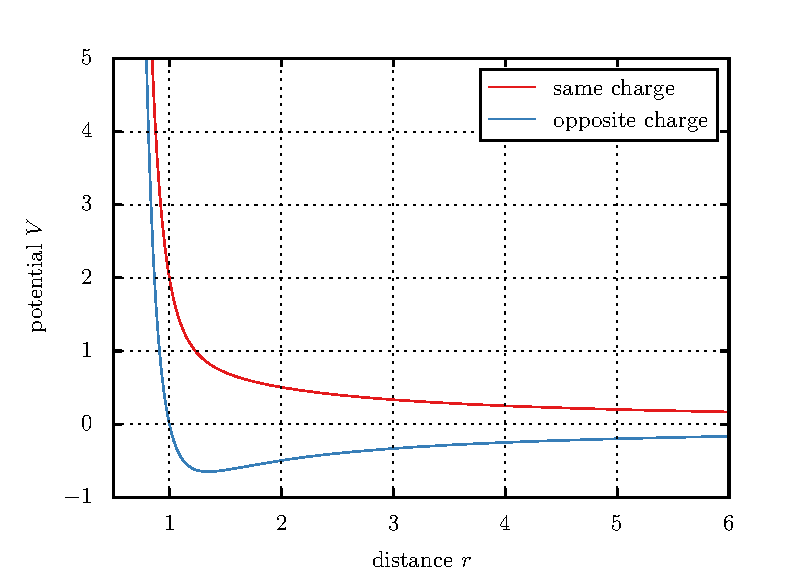
\includegraphics{./figures/potential_coulomb.pdf}
		\subcaption{Coulomb potential with hard core for particles of same and opposite charge.}
		\label{fig:coulomb_core}
	\end{subfigure}
	\begin{subfigure}{1.0\textwidth}
		\centering
		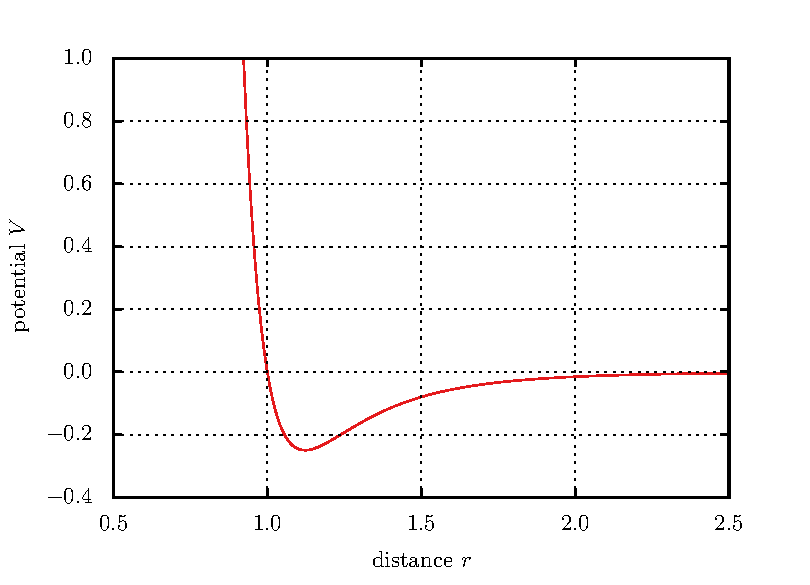
\includegraphics{./figures/potential_lennard_jones.pdf}
		\subcaption{Lennard-Jones potential.}
		\label{fig:lennard_jones}
	\end{subfigure}
	\caption{Inter-particle potentials considered in the simulation of the canonical ensemble.}	
\end{figure}


\subsection{Analysis of the temperature dependence} \label{sec:Temp_Dep}
As already stated the temperature dependence of the canonical ensemble can be monitored using the average pair-distance~$d$ which is given by
\begin{align*}
d = \frac{2}{N(N - 1)} \sum_{i<j} |\mathbf{r}_i - \mathbf{r}_j | \, \text{,}
\end{align*}
where $N$ is the number of particles and $\mathbf{r}_i$, $\mathbf{r}_j$ are the positions of the $i$-th and $j$-th particle.
The calculation of the average pair-distance is only done every 20th step of the Markov-Chain in order to save computation time\footnote{A comparison between the calculation of the observable at every and every 20th step was done and no significant difference in the calculated expectation value was observed.}.
The expectation value of the average pair-distance can then be determined and saved for later analysis.
In order to estimate the uncertainty of the average pair-distance, the standard deviation and 0.05/0.95-quantiles of the expectation values from several chains at the same temperature is used.

In the following sections the average pair-distance~$d$ was simulated for different thermodynamic~$\beta$ and is depicted in $d(\beta)$-graphs using bands to indicate the $1\sigma$-range and quantiles.

\subsubsection{Coulomb potential with hard core in two dimensions} \label{sec:2d_coulomb_tempdep}
For this case a total of 20 positively and 20 negatively charged particles were simulated in a two dimensional box with side length 15.0.
The temperature range of this simulation was chosen to be $\beta \in [1, 500]$, which contains the relevant phase transitions of the ensemble.
Since this range consists of multiple orders of magnitude, the temperature is best depicted using a logarithmic axis.
Therefore the simulated thermodynamic~$\beta$ should increase exponentially to achieve equally spaced points on the logarithmic axis.
Explicitly the simulation starts at $\beta = 1.0$ and increases by approximately \SI{4}{\percent} for each step, which results in a total of 160 simulated temperatures on the range considered.
Moreover for every thermodynamic~$\beta$ a total of \num{4000} chains (with $10^6$ samples each) were generated.

The resulting average pair-distance plot is given in figure \ref{Fig:Temp_dep_Cou2D}, where the red line gives the mean value of the average pair-distance over all chains at a fixed temperature and analogously the red band the range of one standard deviation at either side of the mean.

\begin{figure}[h]
	\centering
	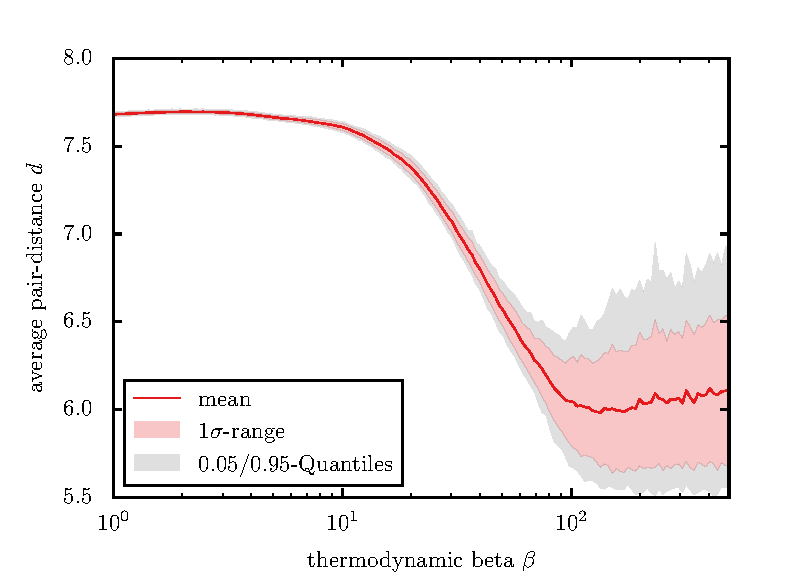
\includegraphics{./figures/temp_dep_coulomb2d.pdf}
	\caption{Temperature dependence of the average pair-distance for a Coulomb potential with hard cores in two dimensions.
		A total of 20 positively and 20 negatively charged particles in a box with side length 15.0 were simulated.}
	\label{Fig:Temp_dep_Cou2D}
\end{figure}

Generally the diagram can be split into three distinct parts, which will be analyzed in the following paragraphs.
For a better understanding one can take a look at the figures in section \ref{sec:Visualisation}.
\begin{description}
	\item[Gaseous state $(\beta \lesssim 10^1)$] 
		The average pair-distance is high for high temperatures or equivalently small $\beta$.
		One expects this behavior, since for high temperatures the system is in a gaseous state and the particles are homogeneously distributed in the whole volume of the box.
		Therefore the average pair-distance is maximum in a gaseous system.
		Moreover one observes small uncertainties in this temperature range because of the homogeneous distribution of the particles.
	
	\item[Liquid state $(10^1 \lesssim \beta \lesssim 10^2)$]
		For higher $\beta$ the average pair-distance decreases.
		This happens at $\beta \approx 10$ at which the system enters a liquid-like state.
		The particles start to form chains, which lead to a reduction in the average pair-distance.
		
		This can be understood if one takes a closer look to equation \ref{Eq:Prob_New_State}.
		The probability that a new proposed state is accepted depends on the value of the thermodynamic~$\beta$.
		With higher $\beta$ the acceptance probability~$\alpha$ gets smaller if a trial state with higher energy is proposed.
		Therefore the Metropolis algorithm tends to minimize the total energy of the state for low temperatures.
		
		In the physical sense this leads to the formation of amorphous structures in a liquid-like state, which tend to reduce the total energy of the system at intermediate temperatures.		
		
	\item[Solid state $(\beta \gtrsim 10^2)$]
		At extremely low temperatures the average pair-distance is almost constant and minimum.
		This is interpreted as the particles forming a lattice and thus entering a solid (crystal-like) state.
		If a regular lattice is formed, the particles cannot get any closer for smaller temperatures, since the particles tend to coincide with the potential minimum as discussed in section \ref{sec:Potentials}.
		
		The reason (concerning the algorithm) that the particles form a solid state with a small average pair-distance is analogous to the argumentation for the liquid state.
		
		Finally one can observe a big uncertainty in figure \ref{Fig:Temp_dep_Cou2D} for the average pair-distance at high $\beta$.
		This is a result of the formation of crystallographic defects in the lattice.
		If the solid is in a state where it is not possible to form a compact grid (due to vacancies or appendices on the crystal), the resulting average pair-distance tends to increase.
		Therefore the formation of crystallographic defects leads to a large uncertainty in the average pair-distance.
\end{description}


\subsubsection{Coulomb potential with hard core in three dimensions}
Similarly to the previous section, the canonical ensemble is simulated using the Coulomb potential between particles with hard cores (still using 20 positively and 20 negatively charged particles).
However this time the particles are considered to be in a three-dimensional box instead of a two-dimensional plane.
To get a particle density that is comparable to the two-dimensional case, the side-length of the box was reduced to \num{8.0}.
The temperature range is unchanged and each simulated chain still contains $10^6$ samples, but the number of chains at each fixed temperature could be reduced to \num{2400} to obtain sufficient results.
The resulting average pair-distance is depicted in figure \ref{fig:temp_dep_cou3d}.
\begin{figure}[h]
	\centering
	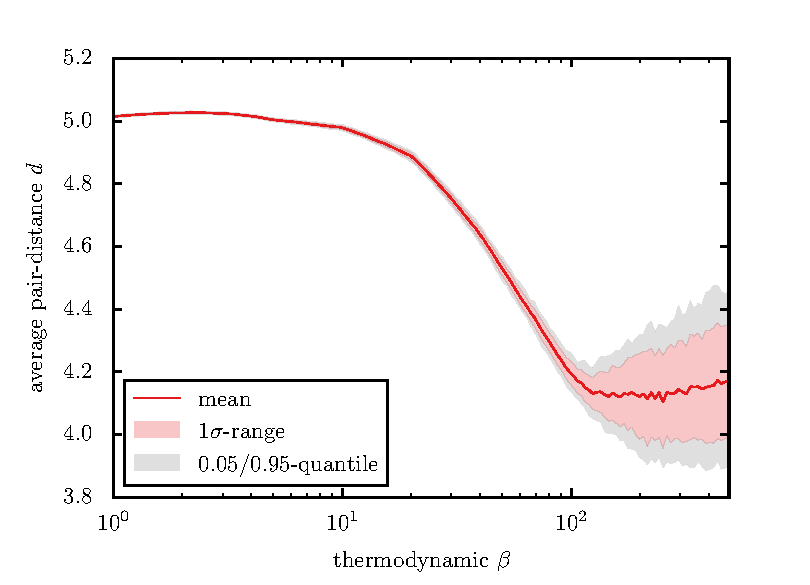
\includegraphics{./figures/temp_dep_coulomb3d.pdf}
	\caption{Temperature dependence of the average pair-distance for a Coulomb potential with hard cores in three dimensions.
		A total of 20 positively and 20 negatively charged particles in a box with side length 8.0 were simulated.}
	\label{fig:temp_dep_cou3d}
\end{figure}

The general behavior of the mean of the average pair-distance is similar to the two-dimensional case.
Therefore the explanations of the phase-transitions of the ensemble transfer to the three-dimensional case.
Nevertheless significant differences in the calculated standard deviations in the low temperature regimes can be observed.
These can be attributed to the additional degree of freedom in the particle's movement, which leads to a higher probability of resolving the crystallographic defects during the formation of a lattice.
Moreover the sphere packing density in three dimensions is bigger than in the two-dimensional case and thus lead to smaller variations in the calculated average pair-distance at low temperatures.


\subsubsection{Two-dimensional case with Lennard-Jones potential}
If the Coulomb potential is exchanged with a Lennard-Jones potential \remark{Gleichung referenzieren} the dependence on $\beta$ changes.
The settings for the plot in figure \ref{Fig:Temp_dep_LJ2D} are basically the same as for the plot in figure \ref{Fig:Temp_dep_Cou2D} but the underlying potential is now a Lennard-Jones potential.
One can clearly see that the behavior for low values of $\beta$ is the same as for the Coulomb potential.
For higher values of $\beta$ the average pair-distance drops.
After the average pair-distance reaches its smallest value it begins to rise again.
%The Lennard-Jones potential has only a short range.
The short range of the Lennard-Jones potential is responsible for this behaviour since some crystal-like state can form but once it has formed it stays on the same place and can not connect with other crystals which are formed somewhere else. \remark{Hier mehr?!}
Some pictures of the final states can be found in section \ref{sec:Visualisation}.

\begin{figure}
	\centering
	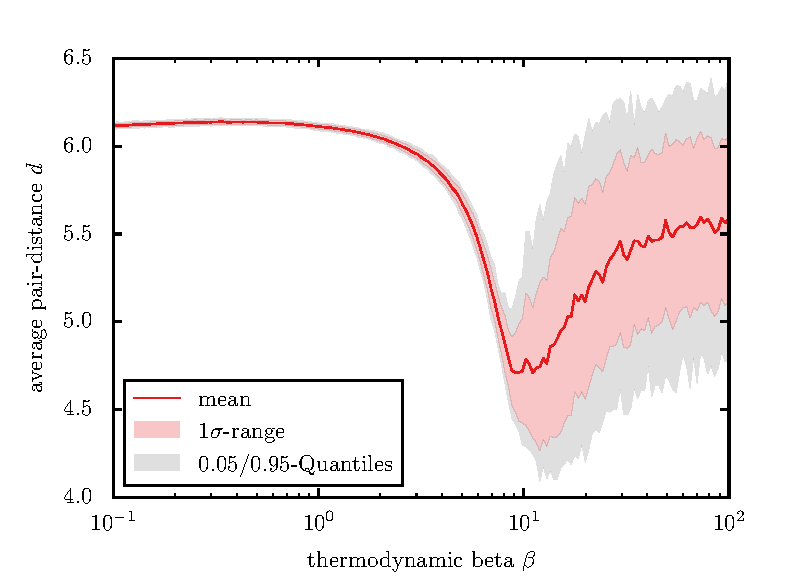
\includegraphics{./figures/temp_dep_lennard_jones2d.pdf}
	\caption{Temperature dependence 3d case \remark{Lennard Jones 2D?}}
	\label{Fig:Temp_dep_LJ2D}
\end{figure}



\subsubsection{Three-dimensional case with Lennard-Jones potential}
\begin{figure}
	\centering
	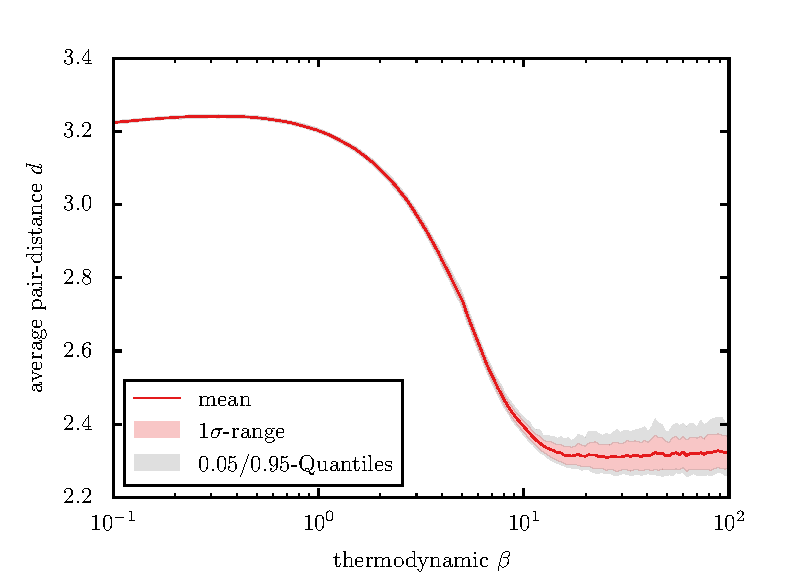
\includegraphics{./figures/temp_dep_lennard_jones3d.pdf}
	\caption{Temperature dependence 3d case \remark{Lennard Jones 2D?}}
	\label{Fig:Temp_dep_LJ3D}
\end{figure}



\subsection{Visualization} \label{sec:Visualisation}
In this section a few examples of the resulting final states are shown.
For each picture a simulation with one million steps was performed.
The position of the particles in the last step were saved and a python script (using the library \texttt{matplotlib}) created an image.

\subsubsection{Two-dimensional case with Coulomb potential} \label{sec:2d_coulomb_vis}

\begin{figure}[p]
	\begin{subfigure}[t]{0.48\textwidth}
		\centering
		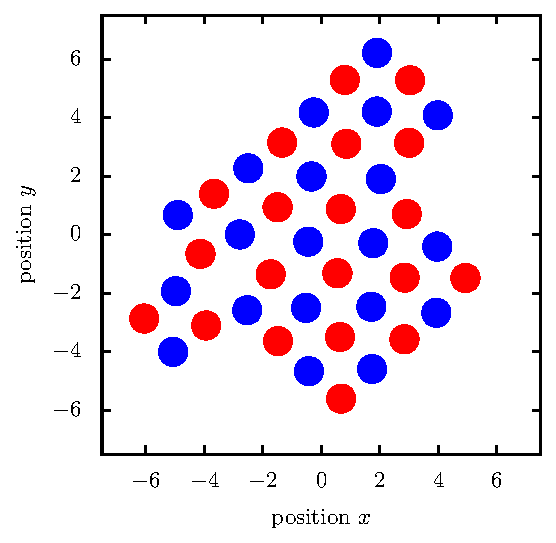
\includegraphics[width=\textwidth]{figures/Kristall_3_beta_500.pdf}
		\subcaption{Final state for $\beta = 500$. 
		One can clearly see that this low temperature leads to a crystal (solid state). 
		The average pair-distance is very small and regularly.
		Another aspect is the quadrangular form of the grid (which is different for the Lennard-Jones potential as shown in 
		Only a few crystallographic defects appear.}
	\end{subfigure}
	\hfill
	\begin{subfigure}[t]{0.48\textwidth}
		\centering
		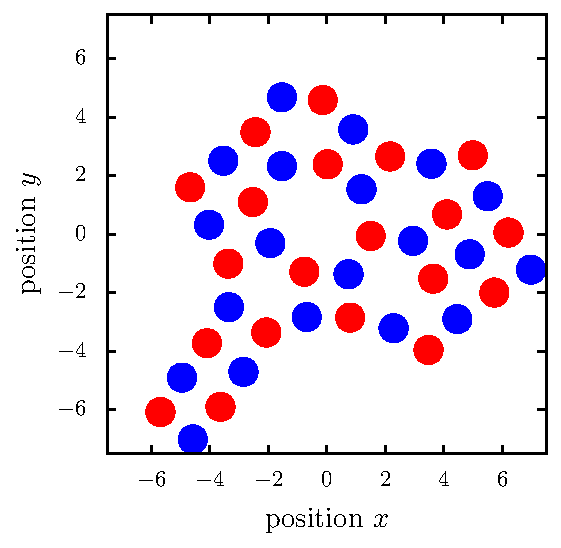
\includegraphics[width=\textwidth]{figures/Kristall_4_beta_500.pdf}
		\subcaption{Final state again for $\beta = 500$. 
		The average pair-distance is slightly larger and the lattice is not regularly.
		A lot of crystallographic defects appear.
		This is the reason for the large uncertainty which was discussed in section \ref{sec:Temp_Dep}.}
	\end{subfigure}
	\begin{subfigure}[t]{0.48\textwidth}
		\centering
		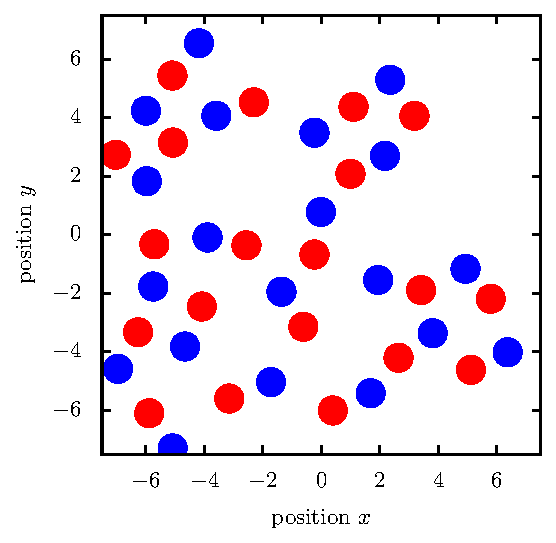
\includegraphics[width=\textwidth]{figures/Fluid_1_beta_40.pdf}
		\subcaption{Final state for $\beta = 40$.
		A higher temperature leads to an amorphous state (fluid).
		The average pair-distance is larger and the lattice is completely gone.
		One can observe some strings and some particles which form a pair.}
	\end{subfigure}
	\hfill
	\begin{subfigure}[t]{0.48\textwidth}
		\centering
		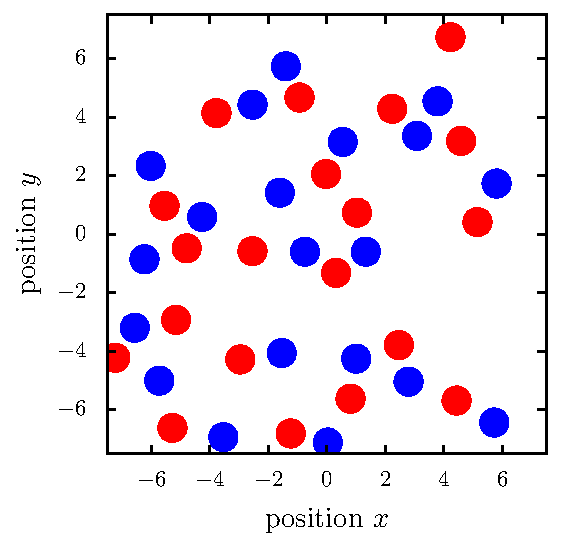
\includegraphics[width=\textwidth]{figures/Gas_1_beta_10.pdf}
		\subcaption{Final state for $\beta = 10$.
		An even higher temperature leads to an gaseous state.
		The average pair-distance is at its maximum since the particles are more or less randomly 		distributed over the whole box.
		Additionally the strings which were observed at the amorphous state are now shorter.
		Often two particles form a pair.}
	\end{subfigure}
	\begin{subfigure}[t]{0.48\textwidth}
		\centering
		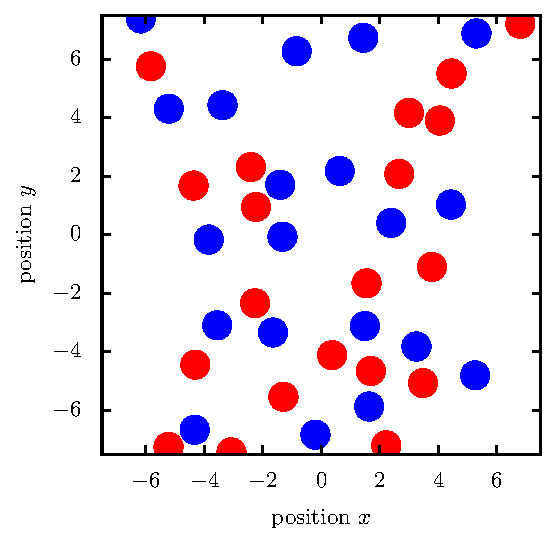
\includegraphics[width=\textwidth]{figures/Plasma_1_beta_2.pdf}
		\subcaption{Final state for $\beta = 2$.
		At very high temperatures the particles are in a plasma-like state since the particles rarely form pairs.
		Sometimes two particles with the same charge are very close together.}
	\end{subfigure}
	\caption{Some pictures}	
\end{figure}

\subsubsection{Two-dimensional case with Lennard-Jones potential}



\begin{figure}[!h]
	\begin{subfigure}[t]{0.48\textwidth}
		\centering
		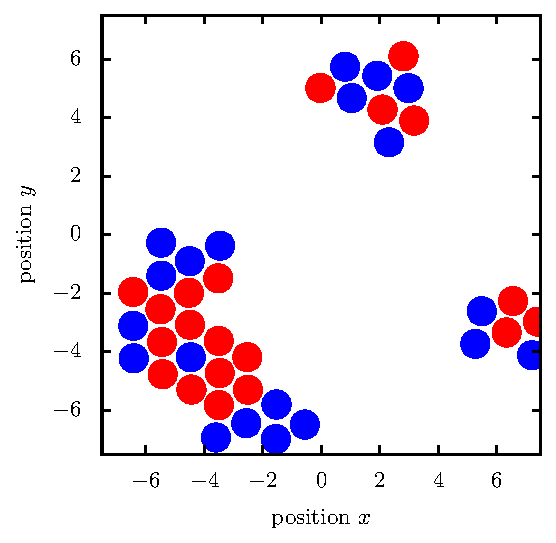
\includegraphics[width=\textwidth]{figures/Beta_100_LJ.pdf}
		\subcaption{Final state for $\beta = 100$.
		As described in section \ref{sec:Temp_Dep} the final state of the system for a high value of $\beta$ is the formation of some small crystals which do not combine since the Lennard-Jones potential has a very short range.
		Another difference compared to the Coulomb potential is the attraction of particles with the same charge.
		The reason is that the Lennard-Jones potential does not depend on the charge.
		Additionally the form of the grid is triangular and not quadrangular as in the Coulomb case.}
	\end{subfigure}
	\hfill
	\begin{subfigure}[t]{0.48\textwidth}
		\centering
		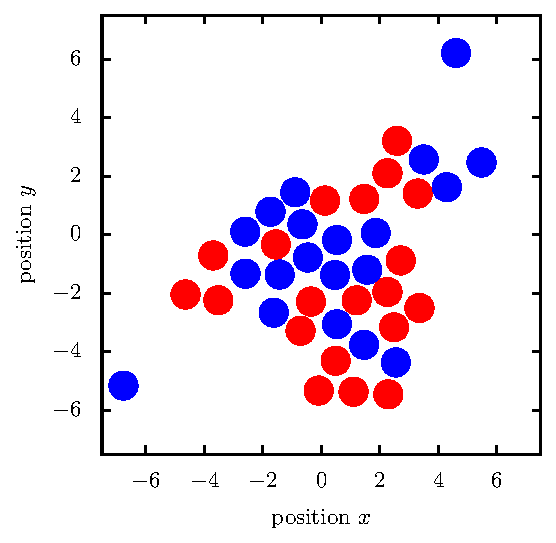
\includegraphics[width=\textwidth]{figures/Beta_10_LJ.pdf}
		\subcaption{Final state for $\beta = 10$.
		Compared with the final state for $\beta=100$ the crystal is now bigger but the structure is more irregular.
		Some particles seem to move freely inside the box.}
	\end{subfigure}
	\begin{subfigure}[t]{0.48\textwidth}
		\centering
		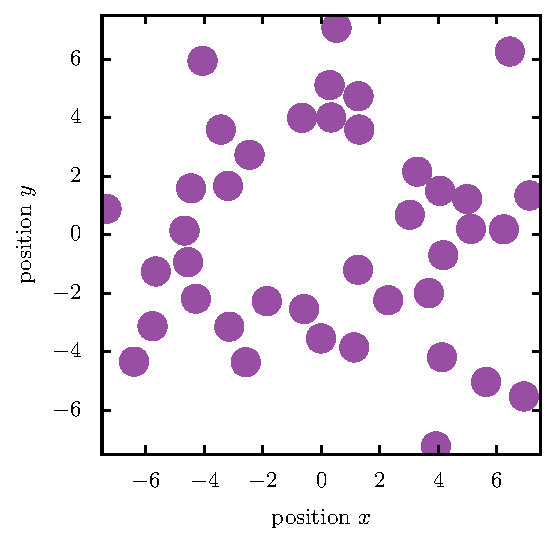
\includegraphics[width=\textwidth]{figures/Beta_5_LJ.pdf}
		\subcaption{Final state for $\beta = 5$.
		This state looks like the state where $\beta = 40$ in the Coulomb case.
		Some particles pair together and form a chain.
		One difference is again the formation of same charged particle pairs.}
	\end{subfigure}
	\hfill
	\begin{subfigure}[t]{0.48\textwidth}
		\centering
		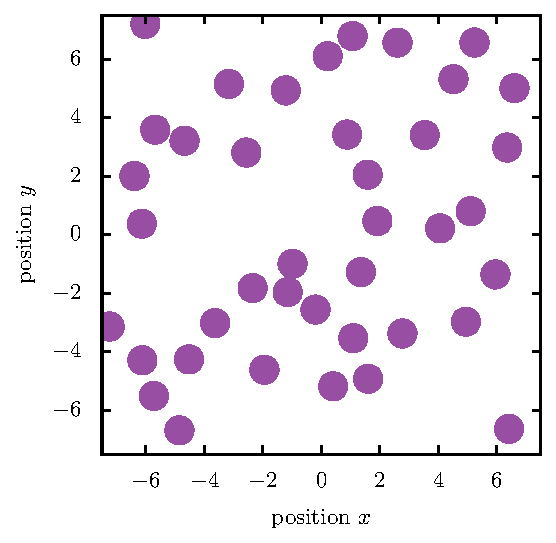
\includegraphics[width=\textwidth]{figures/Beta_1_LJ.pdf}
		\subcaption{Final state for $\beta = 1$.
		The comparison with the final state where $\beta = 2$ in the Coulomb case seems reasonable.
		In both cases are no regularly structures visible and the particles are evenly distributed over the whole box.
		This is again the reason for the small uncertainty of the average pair-distance as shown in figure \ref{Fig:Temp_dep_LJ2D}.}
	\end{subfigure}

\end{figure}


\remark{3D Visualization?}
\section{Further Analysis} \label{sec:Further_Analysis}


\section{Conclusion}

In summary, it can be stated that the project was a success.
The results can be explained with the theory and the written program has worked properly.
But in addition the project will be critically summarized.

\begin{description}
\item[Theory]
The underlying physical theory is not complicated since it is basically the analysis of a potential.
In contrast to that the understanding of the computational physics theory was more difficult.
But, since the idea of this project is to learn more about computational physics, the distribution of the focal points was good.
The suggested algorithm is a good instrument to analyze statistical ensembles how they occur in statistical mechanics.

\item[Implementation]
Once the concept of the Random-Walk Metropolis algorithm was understand, the implementation was not difficult.
The implementation of a very general program was natural.
With this general implementation it was easy to exchange the potentials and to add one more dimension.

\item[Generation of Data]
Since one needs a lot of data to gain reasonable results, this part was a bit lengthy (the total computation time were several days).
But in the end the results are very precise and satisfying therefore the long computation time was a good investment.

\item[Analysis of the Results]
After the data was created it had to be analyzed.
With a few plots and animations one had a good overview about the structure behind the result.
The behavior of the system in dependence of the temperature and the underlying potential can be explained very good.
\end{description}

As a final conclusion this project was very interesting but also challenging.
The learning effect was high due to the high amount of self-reliant work.

\FloatBarrier
% BIBLIOGRAPHY
\vspace{\fill}
\begin{thebibliography}{9}
\bibitem{schwabl}
	F.\ Schwabl,
	\emph{Statistische Mechanik},
	Springer, 3rd edition 2006.

\bibitem{gilks_richardson}
	W.\ R.\ Gilks, S.\ Richardson, D.\ J.\ Spiegelhalter,
	\emph{Markov Chain Monte Carlo in Practice},
	Chapman and Hall/CRC, 1st edition 1995.
\end{thebibliography}

\begin{appendix}
	\newpage
	\section{Source code}
	The full source code can be found on \url{https://github.com/chrisieh/piap} (a \texttt{C++14} compliant compiler is needed).
	\subsection{CanonicalEnsemble{.}h} \label{sec:canonical_ensemble_source}
	\lstinputlisting[language=C++]{../code/src/CanonicalEnsemble.h}
\end{appendix}

\end{document}